\documentclass{article}
\usepackage[T1]{fontenc}
\usepackage{lmodern}
\usepackage{graphicx}
\usepackage{amsmath,amssymb}
\usepackage[a4paper,margin=2cm]{geometry}
\usepackage[absolute,overlay]{textpos}
\setlength{\TPHorizModule}{1mm}
\setlength{\TPVertModule}{1mm}
\usepackage[indonesian]{babel}
\usepackage{hyperref}
\setlength{\emergencystretch}{2em}
% unit: Halaman 63

\begin{document}

% === Halaman 63 (llm) ===

\vspace{163.94mm}

Kegunaan: memeriksa integritas pesan\vspace{10mm}

(Sumber gambar: Wikipedia)

% deskripsi: Diagram yang mengilustrasikan bagaimana perubahan kecil pada pesan input menghasilkan nilai hash kriptografis yang sangat berbeda, menunjukkan sensitivitas fungsi hash terhadap integritas pesan.
% bbox normalisasi: [0.1460, 0.2130, 0.7340, 0.7650]
\begin{textblock*}{123.48mm}(30.66mm,63.26mm)
\noindent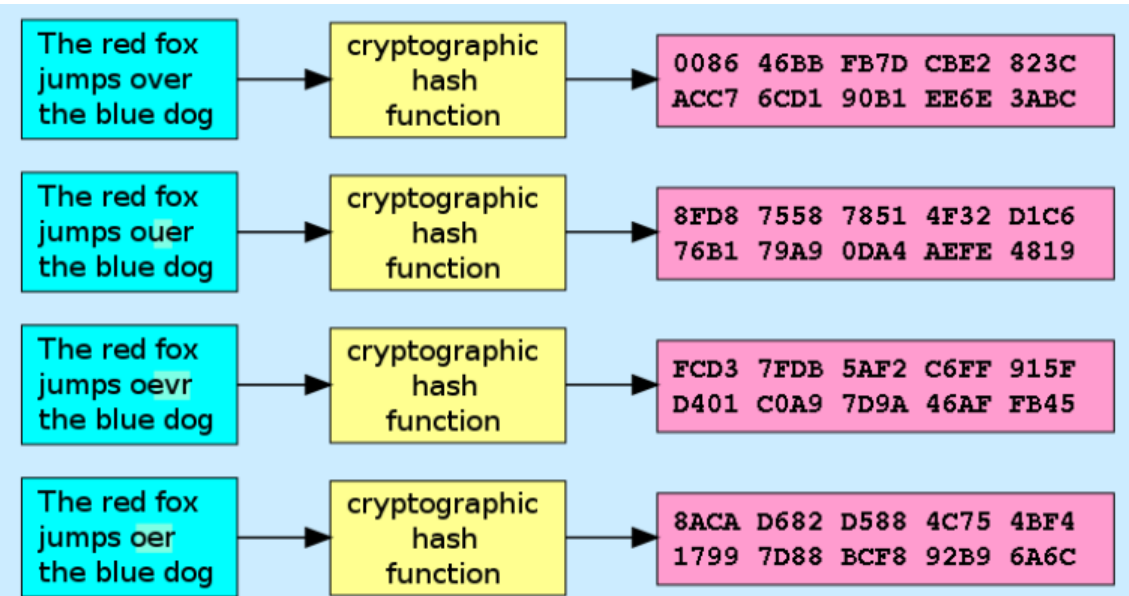
\includegraphics[width=123.48mm,height=163.94mm]{../../images/llm/page_063_img_01.png}%
\end{textblock*}

\end{document}
